\chapter{Project Plan}

% \instructions{
%     Describe the project plan as covered in the SEP2 module. A project plan typically consists of the following topics:
    
%     \begin{itemize}
%         \item Processes, meetings and roles
%         \item Phases, iterations and milestones
%         \item A \textbf{rough} list of things to be done (work items)
%         \item Risk management
%         \item Planning Tools (issue tracker, time tracker, ...)
%     \end{itemize}
    
%     You should \textbf{\underline{not}} describe your \textbf{technical solution} in this chapter. It is all about organizing your project.
% }

\section{Processes}
For the long-term planning we use RUP (\ref{phases}).
For the short-term planning we use Scrum.
The Scrum roles and other assignments are described in \ref{roles}.
The Scrum Events (Sprint Planning, Sprint Review, ...) are declared in \ref{meetings}.
How we implement the Scrum artifacts is defined in \ref{scrum}.

\subsection{Git Workflow}
When working on source code a new branch must be created and before merging the source should be approved by someone other.
Working on the master branch directly is only allowed when the documentation is updated.

\subsection{Scrum}
\label{scrum}
For the short term planning iteration we use the Scrum method.
In the following we describe how we want to implement the Scrum process using GitLab.

\begin{tabular}{l|l}
  \centering
  \textbf{Scrum} & \textbf{GitLab} \\
  \hline
  \textbf{Epic:} & Label with format Epic:xxx \\
  \textbf{User Story / Feature:} & Issues with User Story label \\
  \textbf{Work Item:} & Issue linked to the User Story issue \\
  \textbf{Prioritization:} & Prioritized Labels \\
  \textbf{Story Points:} & Label with format xx\$ \\
  \textbf{Scrum Board:} & Issue Board \\
\end{tabular} \newline

\noindent To build our Scrum Board the following labels are required:

\begin{itemize}
\item ToDo
\item Work in Progress / WIP
\item Done
\end{itemize}

\noindent Work Items issues should not be closed.
However, if the Work Item is finished, then the Label \textsl{Done} should be used.
This approach is used to have an overview per sprint what we have already done.

\noindent To build our Story map the following labels are required \footnote{\url{https://gitlab.ost.ch/SEProj/2022-FS/g03-kubewatch/kubewatch/-/boards/935}}:

\begin{itemize}
\item Epic:xxx
\item User Story
\item Product Backlog
\item Operational
\end{itemize}

\section{Roles}
\label{roles}

\begin{tabular}{l|l}
    \textbf{Role} & \textbf{Person}\\
    \hline
    \textbf{Session Chair:} & Changes every week \\
    \textbf{Product Owner (PO):} & The whole team \\
    \textbf{Developer:} & Benjamin Plattner, Olivier Lischer, Pascal Lehmann\\
    \textbf{Network:} & Jan Untersander, Petra Heeb \\
\end{tabular}
\newline
\noindent The classification in \textsl{Developer} and \textsl{Network} shows only the primary strengths.
Members of the \textsl{Developer} group sometimes also work on the network part and vice versa.


\section{Meetings}
\label{meetings}
We have two weekly meetings: \newline
The first is an internal team meeting every Monday morning is used to implement:
\begin{itemize}
  \item Sprint Planning
  \item Sprint Retrospective 
\end{itemize}

\noindent The second meeting takes place every Tuesday noon with our advisor Laurent Metzger.
In this meeting the \textsl{Sprint Review} is done.
\newline
\noindent The \textsl{Daily Scrum} take places during the week at lunch or during breaks.
One Sprint last between two and four weeks.


\section{Phases, iterations and milestones}
\label{phases}
In our project we work with the four project phases which are defined also in the RUD model which we used for our rough project plan. The four phases are:
\begin{itemize}
    \item Inception
    \item Elaboration
    \item Construction
    \item Transition
\end{itemize}

\subsection{Inception}
The first phase is the \textit{Inception} phase. In this phase we start the new project and  define the following items to plan our project:
\begin{itemize}
    \item Approximate vision
    \item Defining the scope
    \item Rough estimates of efforts
\end{itemize}

\subsection{Elaboration}
The second phase is called \textit{Elaboration}. This phase is used to start the practical part of the project and the goal of this phase is to eliminate potential risks, sometimes using prototypes. There are a few parts we need to handle during this phase:
\begin{itemize}
    \item Identification of most requirements
    \item Iterative implementation of the core architecture
    \item Resolution of high risks
    \item More realistic estimates for efforts
\end{itemize}

\subsection{Construction}
The third and biggest phase is the \textit{Construction} phase. In this phase the team needs to implement the features defined in the project to achieve the product goal. All identified risks should be eliminated by that time or mitigations should be in place to control the risks. The main goal is to have a product ready that can be deployed.
The contents of this phase are:
\begin{itemize}
    \item Iterative implementation of functionality
    \item Resolution of lower risks
    \item Preparation for deployment
\end{itemize}

\subsection{Transition}
The last project phase is called the \textit{Transition} phase during which the project is tested in the whole environment and the project is finished.
The basic elements of this final phase are:
\begin{itemize}
    \item Beta Tests
    \item Deployment
    \item Tie up any loose ends
\end{itemize}

\section{Project Plan}
\subsection{RUD - Rational Unified Process}
To define a rough project plan we use the RUD model which is defined in weekly steps. \newline
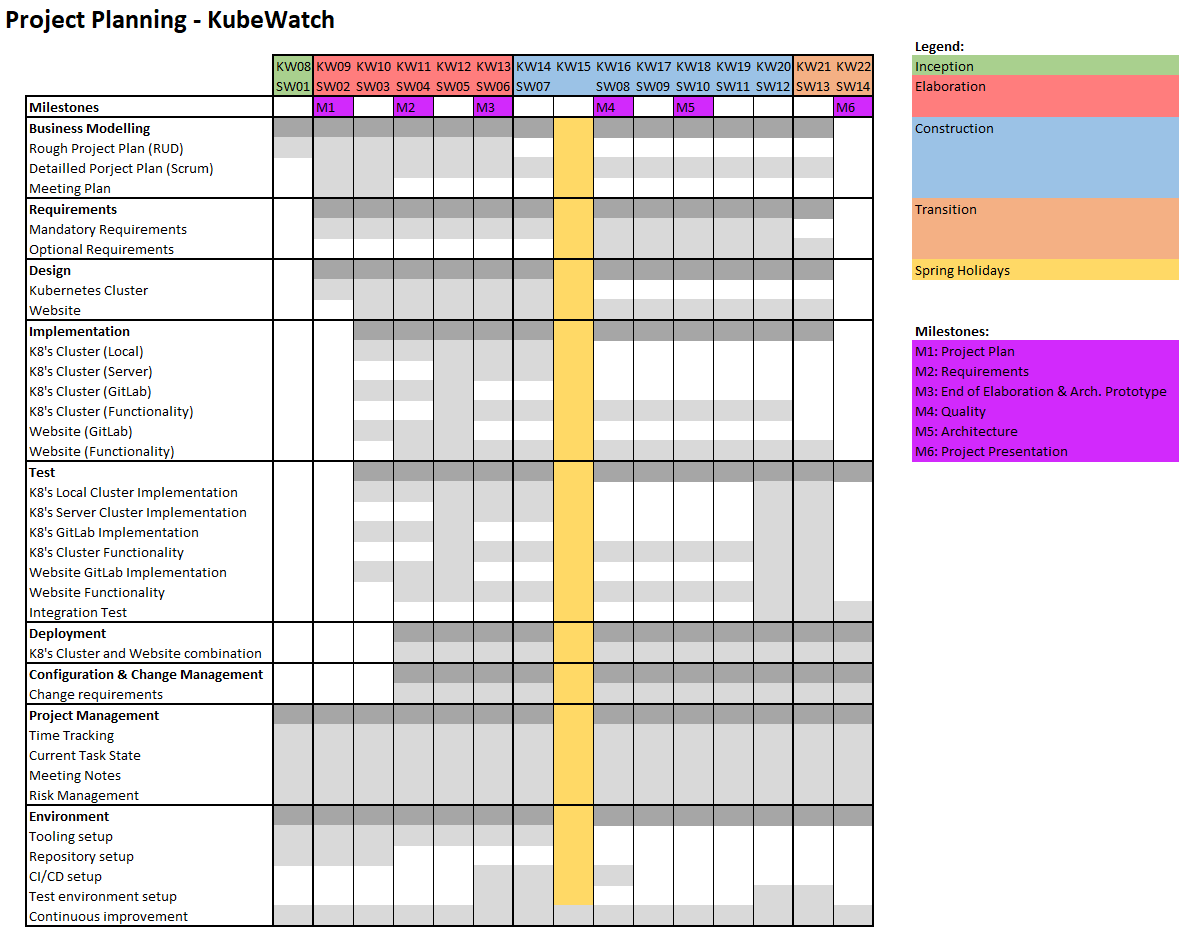
\includegraphics[width=\textwidth]{resources/project-plan-RUD.png}
\newline \newline
The detailed project plan can be found in the projects GitLab repository\footnote{\url{https://gitlab.ost.ch/SEProj/2022-FS/g03-kubewatch/kubewatch/-/tree/main/Documentation/src/03_project-documentation}}.

\section{Planning Tools}
For planning our work, issue handling and time tracking we use GitLab issues, merge requests and the built-in time tracking functionality.

\section{Risk Management}

As part of a continuing risk management analysis, we use a risk matrix to estimate the impact of the identified risks.\newline
Figure \ref{fig:risk-matrix} presents an overview of the categorisation of the identified risks.

\subsection{Risk Methodology}
We use a risk weighted approach to estimate the impact of a new risk. The impact is calculated as the product of the 'severity of the damage', which is a category of scale 1 to 10, and the 'probability of occurrence'. To better gauge the severity of damage, we use a relativistic approach where we compare existing risks with new risks and decide on the relative impact one risk has versus others.

\subsection{Risk Review Process}
The identification and analysis of new risks happen continuously, but at least once every new sprint. There, the team discusses potential new risks and one team member is then assigned to update the documentation accordingly.

The table \ref{tab:risk-review} lists all risk reviews.

\begin{table}[h!]
\centering
  \caption{\label{tab:risk-review}All Risk Reviews}
  \begin{tabular}{ | l | l | }
    \hline
    \textbf{Date} & \textbf{Changes} \\
    \hline
    03.03.22 & Created initial analysis. \\
    \hline
    14.03.22 & Risk reviewed. Added  changed. \\
    \hline
  \end{tabular}
\end{table}

\begin{figure}[h]
    \centering
    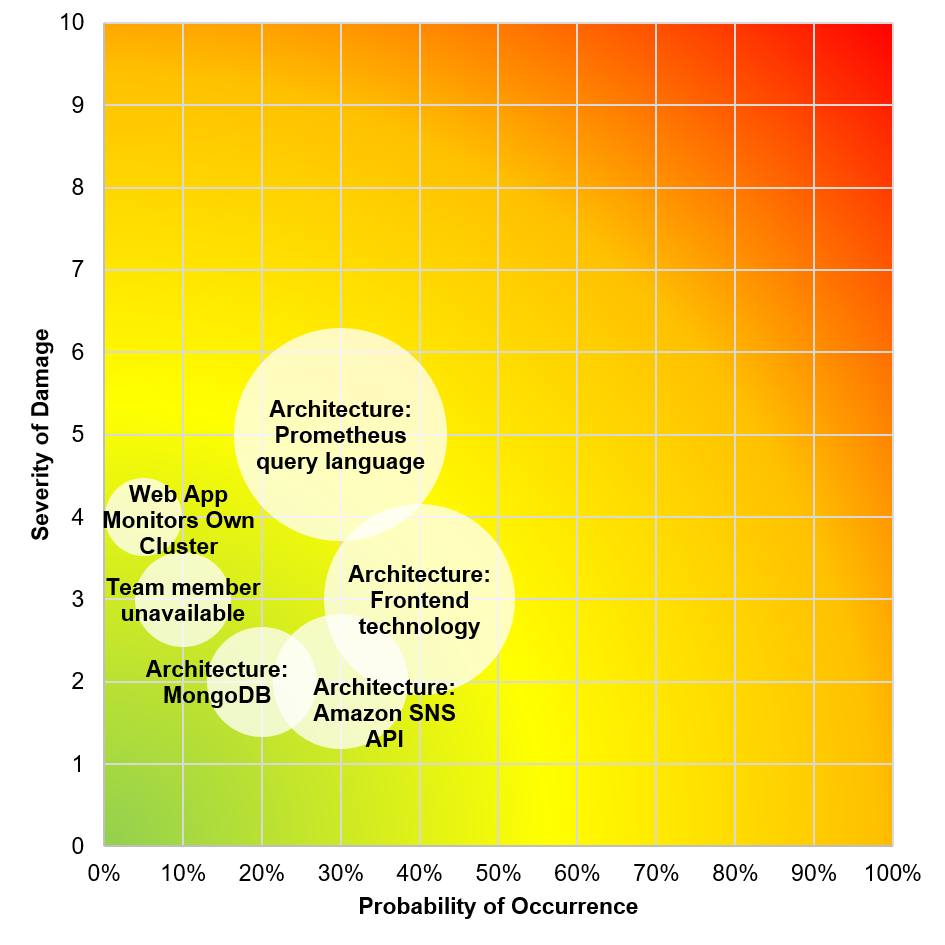
\includegraphics[width=11cm]{resources/risk_matrix.png}
    \label{fig:risk-matrix}
\end{figure}


% \begin{landscape}
\label{tab:risk-classification}
    %\begin{tabular*}{\textwidth}{ p{2.2cm} | p{5cm} | p{5cm} | p{2.0cm} | p{2.0cm} | p{2.0cm} }
% \begin{longtable}{@{\extracolsep{\fill}}c c c c c c@{}}
\begin{longtable}[h]{p{2.2cm} | p{4cm} | p{4cm} | p{1.5cm} | p{1.5cm} | p{1.5cm}}
    \caption{Classification of identified risks} \\
    \textbf{Risk Name} & \textbf{Risk Description} & \textbf{Mitigation} & \textbf{Probability of Occurrence} & \textbf{Severity of Damage (0-10)} & \textbf{Weighted Damage} \\ \hline
    \endhead
        Kubernetes Cluster
            & The deployment and setup of the Kubernetes Cluster has only been performed by Petra and Jan as part of their Cloud Infrastructure class. It may take a long time to fully configure the desired setup.
            & With the help of the INS we can leverage their expertise in setting up K8s clusters and apply default configurations.
            & \multicolumn{1}{c}{Eliminated} \\ \hline
        Unknown API 
            & The API to extract data points from the K8s cluster is new to us. There are libraries like Prometheus which can collect such data, but we do not have much experience using it.
            & As a first step we investigated the API and did a few preliminary test to see how it works. The results were positive but we may need to do more tests when the architecture is further refined.
            & 60\% & 5 & 3 \\ \hline
        Accessing K8s Cluster 
            & To access the K8s Cluster that is set up in the INS, we need to define the best way for everyone to work on the Cluster and subsequently the Web API.
            & The INS has different options to access the cluster, but we have not yet been able to test it.
            & 40\% & 8 & 3.2 \\ \hline
        Unknown Development Environment
            & To run a Web Server on a K8s Cluster is new for us and may come with certain obstacles which would not appear in a local development environment. However, the tech stack we are planning on using is well known to us.
            & Test the K8s development environment as soon as possible and stick to tutorials for setting up Web services on a K8s Node. This has been achieved by others before, and since we are not using a highly customised K8s setup, other use cases may help us with troubleshooting if necessary.
            & 60\% & 7 & 4.2 \\ \hline
        Scrum Methodology 
            & We are applying an Agile approach for the development of this project. The Scrum framework is best suited for us as it has clear guidelines. However, we do not have much experience in running Scrum methodologies.
            & The Software Engineering Project module, which we attend in parallel, is designed to support us in learning and applying Scrum. Also, we help each other out with running Scrum meetings. The impact of not fully conforming with the Scrum methodology should not have a massive impact on the final product as we can improve our processes with each iteration.
            & 40\% & 1 & 0.4 \\ \hline
        New Architecture 
            & Designing a new architecture for a project for which we have on prior experience is always a risk that something gets overlooked.
            & The architecture for our desired final state of the project is not overly complex. Also, we have experience with the individual components that we intend to use, just not in combining them in the desired setup. However, the available documentations are fairly extensive and keeping the architecture simple is key. Once the architecture is finalised, we should have a better grasp of how comfortable we feel with implementing it.
            & 80\% & 8 & 6.4 \\ \hline
        Team member unavailable
            & One or more team members may become unavailable for the project due to illness, accident or other personal reasons. In this case, the workload must be spread across fewer members, which has an impact on the timeline. Also, information may get lost that was only available to that person.
            & Information sharing across team members is important. We formed two sub-groups (Network and Web development) where information is shared, and we train each other during the weekly meetings on important developments. In addition, we maintain a practice of documenting code and other implementation specific details in a shared repository. Thanks to an agile approach, change in timelines only impact the number of features available in the final product, rather than posing a threat to the success of the overall project.
            & 10\% & 3 & 0.3 \\ \hline
        Web App Monitors Own Cluster
            & The Web Application that monitors the Kubernetes Cluster runs on the same Cluster which it monitors. This may become a risk if the Cluster or Node where the app runs unexpectedly goes down, so that a notification cannot be sent before the shutdown.
            & We are aware of this issue and constantly monitor the Cluster while development is ongoing. Once in production, the app should then reside on a separate Cluster.
            & 5\% & 8 & 0.4 \\ \hline
    %\end{tabular*}
\end{longtable}
% \end{center}
% \end{landscape}
% \restoregeometry
